\chapter{ทฤษฎีที่เกี่ยวข้อง}
ในบทนี้จะอธิบายถึงองค์ความรู้และทฤษฎีที่จำเป็นต่อการพัฒนาแอปพลิเคชันรวมทั้งงานวิจัยที่เกี่ยวข้อง มีรายละเอียดดังนี้
\begin{enumerate}[label=2.\arabic*]
	\item Hybrid Mobile Application
	\item ความรู้พื้นฐานระบบปฏิบัติการแอนดรอยด์
	\item ความรู้พื้นฐานของระบบปฏิบัติการไอโอเอส
	\item ความรู้พื้นฐาน Ionic Framework
	\item การใช้งาน Firebase เป็นฐานข้อมูล
	\item ความรู้พื้นฐานของแชทบอท
	\item Dialogflow
	\item Libraries moment.js
	\item Google Maps API
	\item เอกสารและงานวิจัยที่เกี่ยวข้อง
\end{enumerate}

\section{Hybrid Mobile Application}

\begin{figure}[H]
	\centering
	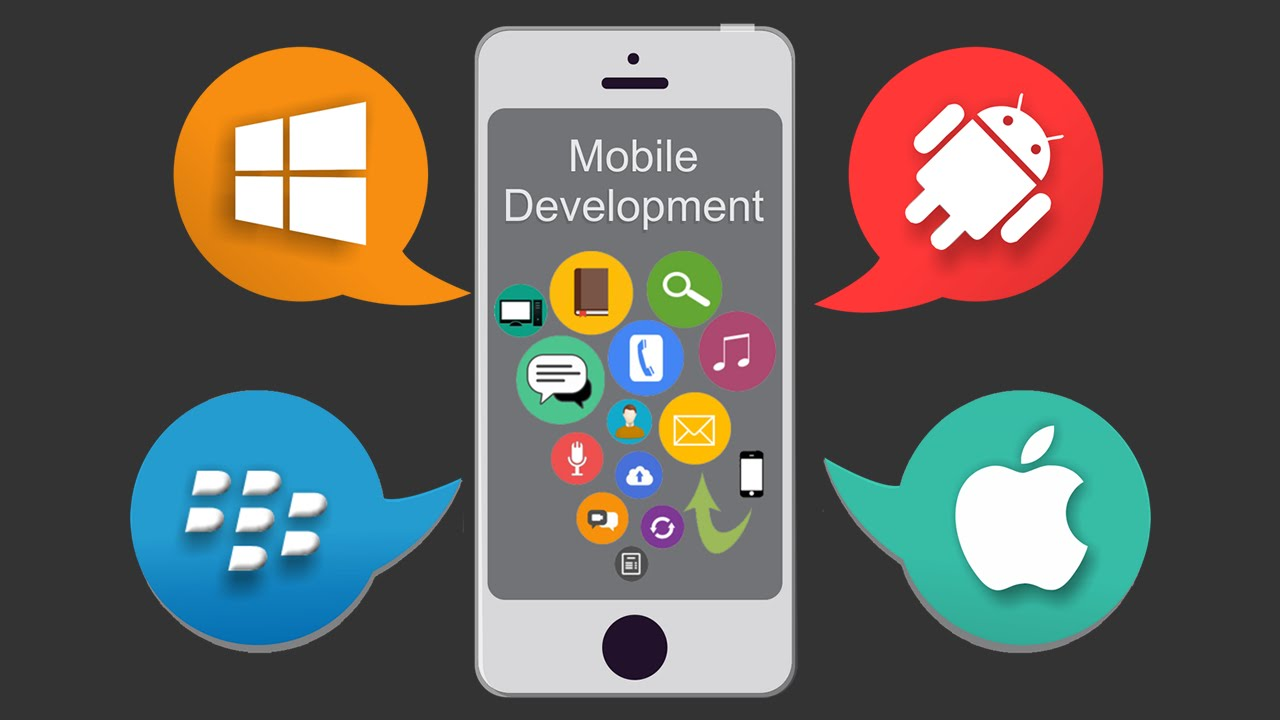
\includegraphics[width=0.5\columnwidth]{Figures/2/hybrid}
	\caption{Hybrid Mobile Application คืออะไร}{ที่มา :  https://www.mindphp.com/คู่มือ/73-คืออะไร/3663-hybrid-application-ไฮบริด-แอปพลิเคชัน-หรือ-hybrid-app-ไฮบริด-แอพ-คืออะไร.html}
	\label{Fig:maketshare}
\end{figure}

Hybrid Application คือ แอปพลิเคชันที่ถูกพัฒนาขึ้นมาเพื่อให้สามารถทำงานได้บนระบบปฏิบัติการทั้งหมดโดยพัฒนาแค่ครั้งเดียว 
โดยจำเป็นต้องผ่านเฟรมเวิร์คต่างๆเพื่อให้สามารถทำงานบน OS นั้นๆได้ เช่น PhoneGap (โฟนเคป) ซึ่งเป็น Open source framework 
ด้วยการพัฒนาแอปด้วยเทคโนโลยีเว็บ html, CSS และ Java Script เป็นต้น 

การพัฒนา Mobile Application แต่เดิมนั้น ถ้าจะเริ่มก็คงตั้งแต่ยุค J2ME อาจจะเก่ามากจนมาถึงยุคสมัยของ IOS และ Android 
รวมไปถึงน้องสุดท้องอย่าง Windows Phone 
ซึ่งแต่ก่อนก็มีพัฒนาจาก Window CE มาก่อนหน้านี้ จนผู้ใช้ของแต่ละฝั่ง platform เริ่มมีความสำคัญใกล้เคียงกัน ดังนั้น การพัฒนาแอป
เฉพาะของ iOS หรือ Android เพียงอย่างเดียวถือเป็นการเสียโอกาสทางธุรกิจเป็นอย่างมาก จนมีคนเริ่มคิดหาวิธีทำให้ชีวิตง่ายขึ้นโดยการเขียน 
HTML5 + CSS3 + JavaScript แล้วใช้วิธีทำงานผ่าน Web View Component เป็นส่วนของหน้าเบราเซอร์ในแอปอีกที ของแต่ละ Platform 
จนกลายมาเป็นโครงการ Cordova และได้มีการพัฒนาส่วนขยาย Plug-In เพิ่มเรื่อยๆ ทำให้ปัจจุบันเราสามารถเข้าถึง Hardware หรือ Sensor 
ซึ่งโดยปกติ HTML5 ธรรมดาไม่สามารถเข้าถึงได้ 

จากได้อ่านส่วนบนมา การเขียนแอปแบบ Hybrid Application คือ การพัฒนาแ โดยอาศัย Framwork หรือ SDK 
ที่ถูกสร้างมาจากหลากหลายภาษาและมีเครื่องมือที่เหมาะสมกับ Framwork หรือ SDK นั้น ๆ ให้เลือกใช้ในการพัฒนาที่หลากหลายตัวอย่างเช่น 
codova SDK ใช้ ภาษา LUA , Acrobat AIR ใช้ภาษา ACTION SCRIPT 3 หรือ UNITY ใช้ C# และ JAVASCRIPT 
ซึ่งการเขียนในรูปแบบนี้เราสามารถแปลงไปใช้กับระบบปฏิบัติการอื่น ๆ ได้และใช้เวลาน้อยในการเพื่อพัฒนาหลาย ๆ แอปพลิเคชัน

	\subsection{ข้อดีของ Hybrid Mobile Application}
	\begin{enumerate}
		\item พัฒนาด้วยภาษา HTML, CSS และ JavaScript ทำให้ง่ายและเรียนรู้ได้อย่างรวดเร็ว
		\item พัฒนาครั้งเดียวสามารถใช้ได้หลาย Platform ทั้ง iOS, Android และ Window Phone
		\item ใช้ต้นทุนในการพัฒนาน้อยกว่า Native App
	\end{enumerate}

	\subsection{ข้อเสียของ Hybrid Mobile Application}
	\begin{enumerate}
		\item ประสิทธิภาพการทำงานจะด้อยกว่า Native App
		\item ในบางกรณีอาจจะใช้ความสามารถของอุปกรณ์ได้ไม่เต็มที่ เนื่องจากต้องขึ้นอยู่กับ Framework ที่เลือกในการพัฒนานั้นมี Component ที่ต้องการหรือไม่
		ดังนั้น Hybrid App จึงมีจุดเด่นในเรื่องความง่ายและพัฒนาได้รวดเร็ว และ Cross-Platforms คือพัฒนาครั้งเดียวแต่สามารถนำไปติดตั้งในหลาย Platforms แต่เมื่อพูดถึงเรื่องประสิทธิภาพในการทำงาน เช่นความเร็ว หรือการเรียกใช้หรือติดต่อ feature ต่าง ๆ ของอุปกรณ์ ก็ต้องยอมรับว่าอาจจะยังด้อยกว่าแอปพลิเคชันที่พัฒนาด้วย Native App ในบางลักษณะการทำงานอยู่ดี
	\end{enumerate}

\section{ความรู้พื้นฐานระบบปฏิบัติการแอนดรอยด์}
	แอนดรอยด์ (Android) คือระบบปฏิบัติการแบบเปิดเผยซอร์ฟแวร์ต้นฉบับ (Open Source) โดยบริษัท กูเกิ้ล (Google Inc.) ที่ได้รับความนิยมเป็นอย่างสูง เนื่องจากอุปกรณ์ที่ใช้ระบบปฏิบัติการแอนดรอยด์ มีจำนวนมาก อุปกรณ์มีหลากหลายระดับ หลายราคา รวมทั้งสามารถทำงานบนอุปกรณ์ที่มีขนาดหน้าจอ และความละเอียดแตกต่างกันได้ ทำให้ผู้บริโภคสามารถเลือกได้ตามต้องการและหากมองในทิศทางสำหรับนักพัฒนาโปรแกรม (Programmer) แล้วนั้นการพัฒนาโปรแกรมเพื่อใช้งานบนระบบปฏิบัติการแอนดรอยด์ ไม่ใช่เรื่องยาก เพราะมีข้อมูลในการพัฒนารวมทั้ง Android SDK (Software Development Kit) เตรียมไว้ให้กับนักพัฒนาได้เรียนรู้ และเมื่อนักพัฒนาต้องการจะเผยแพร่หรือจำหน่ายโปรแกรมที่พัฒนาแล้วเสร็จแอนดรอยด์ก็ยังมีตลาดในการเผยแพร่โปรแกรม Google PlayStore แต่หากจะกล่าวถึงโครงสร้างภาษาที่ใช้ในการพัฒนานั้น สำหรับ Android SDK จะยึดโครงสร้างของภาษาจาวา (Java language) ในการเขียนโปรแกรม เพราะโปรแกรมที่พัฒนามาได้จะต้องทำงานอยู่ภายใต้ Dalvik Virtual Machine เช่นเดียวกับโปรแกรมจาวา ที่ต้องทำงานอยู่ภายใต้ Java Virtual Machine (Virtual Machine เปรียบได้กับสภาพแวดล้อมที่โปรแกรมทำงานอยู่)
	
	นอกจากนี้แล้วแอนดรอยด์ยังมีโปรแกรมแกรมที่เปิดเผยซอร์ฟแวร์ต้นฉบับ (Open Source) เป็นจำนวนมาก ทำให้นักพัฒนาที่สนใจสามารถนำซอร์ฟแวร์ต้นฉบับมาศึกษาได้ประกอบกับความนิยมของแอนดรอยด์ได้เพิ่มขึ้นอย่างมากในปัจจุบัน โดยดูได้จากส่วนแบ่งการตลาด ดังรูปที่ \ref{Fig:maketshare}
	
	\begin{figure}[H]
		\centering
		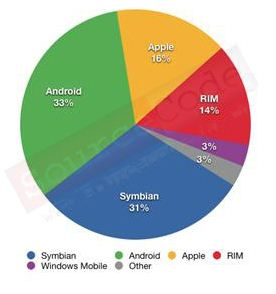
\includegraphics[width=0.5\columnwidth]{Figures/2/maketshare}
		\caption{ส่วนแบ่งการตลาดระบบปฏิบัติการบนสมาร์ทโฟน}{ที่มา :  https://beerkung.wordpress.com/ระบบปฏิบัติการรุ่นล่าส/ระบบปฏิบัติการ-android.html}
		\label{Fig:maketshare}
	\end{figure}

	\subsection{ประวัติความเป็นมาของระบบปฏิบัติการแอนดรอยด์}
	เริ่มต้นระบบปฏิบัติการแอนดรอยด์ถูกพัฒนามาจากบริษัทแอนดรอยด์ (Android) เมื่อปี พ.ศ 2546 โดยมีนาย แอนดี้ รูบิน (Andy Rubin) ผู้ให้กำเนิดระบบปฏิบัติการนี้และถูกบริษัทกูเกิ้ลเข้าซื้อกิจการเมื่อ เดือนสิงหาคม ปี พ.ศ 2548 โดยบริษัทแอนดรอยด์ ได้กลายมาเป็นบริษัทลูกของบริษัทกูเกิ้ล
	
	ระบบปฏิบัติการแอนดรอยด์ เป็นระบบปฏิบัติการที่พัฒนามาจากการนำเอาแกนกลางของระบบปฏิบัติการลินุกซ์ (Linux Kernel) ซึ่งเป็นระบบปฏิบัติการที่ออกแบบมาเพื่อทำงานเป็นเครื่องให้บริการ (Server) มาพัฒนาต่อ เพื่อให้กลายเป็นระบบปฏิบัติการบนอุปกรณ์พกพา (Mobile Operating System)
	
	ต่อมาเมื่อเดือน พฤศจิกายน ปี พ.ศ 2550 บริษัทกูเกิ้ล ได้ทำการก่อตั้งสมาคม OHA (Open Handset Alliance) เพื่อเป็นหน่วยงานกลางในการกำหนดมาตรฐานกลาง ของอุปกรณ์พกพาและระบบปฏิบัติการแอนดรอยด์ โดยมีสมาชิกในช่วงก่อนตั้งจำนวน 34 รายเข้าร่วม ซึ่งประกอบไปด้วยบริษัทชั้นนำที่ดำเนินธุรกิจด้าการสื่อสาร เช่น โรงงานผลิตอุปกรณ์พกพา บริษัทพัฒนาโปรแกรม ผู้ให้บริการสื่อสาร และผู้ผลิตอะไหล่อุปกรณ์ด้านสื่อสาร   \cite{openhandsetalliance}
	
	หลังจากนั้น เมื่อเดือนตุลาคม ปี พ.ศ 2551 บริษัท กูเกิ้ล ได้เปิดตัวมือถือตัวแรกที่ใช้ระบบปฏิบัติการแอนดรอยด์ ที่ชื่อ T-Mobile G1 หรืออีกชื่อนึงคือ HTC Dream โดยใช้แอนดรอยด์รุ่น 1.1 และหลังจากนั้น ได้มีการปรับพัฒนาระบบปฏิบัติการเป็นรุ่นใหม่ มาเป็นลำดับ
	
	ช่วงต่อมาได้มีการออกผลิตภัณฑ์จากบริษัทต่าง ๆ ออกมาหลากหลายรุ่น หลากหลายยี่ห้อ ตามการพัฒนาระบบปฏิบัติการแอนดรอยด์ ที่มีอยู่อย่างต่อเนื่อง ทำให้สินค้าของแอนดรอยด์ มีให้เลือกอยู่อย่างมากมาย
	
	\subsection{โครงสร้างของระบบปฏิบัติการแอนดรอยด์}
	การทำความเข้าใจโครงสร้างของระบบปฏิบัติการแอนดรอยด์ \cite{androidbook1} ถือว่าเป็นสิ่งสำคัญเพราะถ้านักพัฒนาโปรแกรม สามารถมองภาพโดยรวมของระบบได้ทั้งหมด จะสามารถเข้าใจถึงกระบวนการทำงานได้ดียิ่งขึ้น และสามารถนำไปช่วยในการออกแบบโปรแกรมที่ต้องการพัฒนาเพื่อให้เกิดประสิทธิภาพในการทำงาน
	
	\begin{figure}[H]
		\centering
		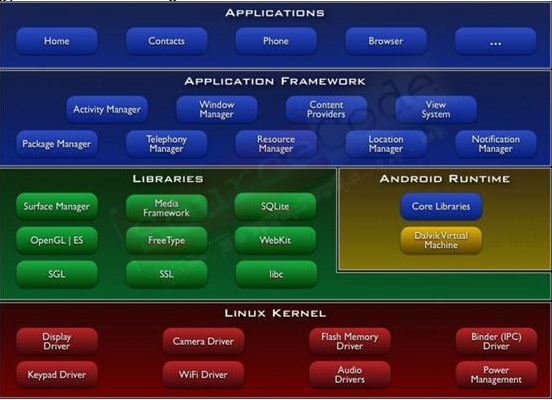
\includegraphics[width=0.8\columnwidth]{Figures/2/androidarchitecture}
		\caption{โครงสร้างของระบบปฏิบัติการแอนดรอยด์}{ที่มา : https://www.theandroid-mania.com/android-architecture/}
		\label{Fig:androidarchitecture}
	\end{figure}
	จากโครงสร้างของระบบปฏิบัติการแอนดรอยด์ในรูปที่ \ref{Fig:androidarchitecture} จะสังเกตได้ว่า มีการแบ่งออกเป็นส่วน ๆ ที่มีความเกี่ยวเนื่องกัน โดยส่วนบนสุดเป็นส่วนที่ผู้ใช้งานทำการติดต่อโดยตรงซึ่งคือส่วนของ Applications ลำดับถัดมาเป็นองค์ประกอบอื่น ๆ ตามลำดับ และสุดท้ายเป็นส่วนที่ติดต่อกับอุปกรณ์โดยผ่านทาง Linux Kernel โครงสร้างของแอนดรอยด์สามารถอธิบายได้ดังนี้

	\begin{enumerate}
		\item Applications ส่วนแอปพลิเคชันหรือส่วนของโปรแกรมที่มากับระบบปฏิบัติการ หรือเป็นกลุ่มของโปรแกรมที่ผู้ใช้งานได้ทำการติดตั้งไว้ โดยผู้ใช้งานสามารถเรียกใช้โปรแกรมต่าง ๆ ได้โดยตรงซึ่งการทำงานของแต่ละโปรแกรมจะเป็นไปตามที่ผู้พัฒนาโปรแกรมได้ออกแบบและเขียนโค้ด (Code) โปรแกรมเอาไว้
		\item Application Framework  เป็นส่วนที่มีการพัฒนาขึ้นเพื่อให้นักพัฒนาสามารถพัฒนาโปรแกรมได้สะดวก และมีประสิทธิภาพมากยิ่งขึ้น โดยนักพัฒนาไม่จำเป็นต้องพัฒนาในส่วนที่มีความยุ่งยากมากๆ เพียงแค่ทำการศึกษาถึงวิธีการเรียกใช้งาน Application Framework ในส่วนที่ต้องการใช้งานแล้วนำมาใช้งาน ซึ่งมีหลายกลุ่มด้วยกัน ตัวอย่างเช่น
			\begin{itemize}
				\item Activities Manager เป็นกลุ่มของชุดคำสั่งที่จัดการเกี่ยวกับวงจรการทำงานของหน้าต่างโปรแกรม (Activity)
				\item Content Providers เป็นกลุ่มของชุดคำสั่ง ที่ใช้ในการเข้าถึงข้อมูลของโปรแกรมอื่น และสามารถแบ่งปันข้อมูลให้โปรแกรมอื่นเข้าถึงได้
				\item View System เป็นกลุ่มของชุดคำสั่งที่เกี่ยวกับการจัดการโครงสร้างของหน้าจอที่แสดงผลในส่วนที่ติดต่อกับผู้ใช้งาน (User Interface)
				\item Telephony Manager เป็นกลุ่มของชุดคำสั่งที่ใช้ในการเข้าถึงข้อมูลด้านโทรศัพท์ เช่น หมายเลขโทรศัพท์ เป็นต้น
				\item Resource Manager เป็นกลุ่มของชุดคำสั่งในการเข้าถึงข้อมูลที่เป็นข้อความและรูปภาพ
				\item Location Manager เป็นกลุ่มของชุดคำสั่งที่เกี่ยวกับตำแหน่งทางภูมิศาสตร์ที่ระบบปฏิบัติการได้รับค่าจากอุปกรณ์
				\item Notification Manager เป็นกลุ่มของชุดคำสั่งที่จะถูกเรียกใช้เมื่อโปรแกรมต้องการแสดงผลให้กับผู้ใช้งาน ผ่านทางแถบสถานะ (Status Bar) ของหน้าจอ
			\end{itemize}
		\item Libraries เป็นส่วนของชุดคำสั่งที่พัฒนาด้วย C/C++ โดยแบ่งชุดคำสั่งออกเป็นกลุ่มตามวัตถุประสงค์ของการใช้งาน เช่น Surface Manage จัดการเกี่ยวกับการแสดงผล Media Framework จัดการเกี่ยวกับการการแสดงภาพและเสียง Open GL|ES และ SGL จัดการเกี่ยวกับภาพ 3 มิติ และ 2 มิติ SQLlite จัดการเกี่ยวกับระบบฐานข้อมูล เป็นต้น
		\item Android Runtime จะมี Darvik Virtual Machine ที่ถูกออกแบบมาเพื่อให้ทำงานบนอุปกรณ์ที่มีหน่วยความจำ (Memmory) หน่วยประมวลผลกลาง (CPU) และพลังงาน (Battery) ที่จำกัดซึ่งการทำงานของ Darvik Virtual Machine จะทำการแปลงไฟล์ที่ต้องการทำงานไปเป็นไฟล์ .DEX ก่อนการทำงานเหตุผลเพื่อให้มีประสิทธิภาพเพิ่มขึ้นเมื่อใช้งานกับหน่วยประมวลผลกลางที่มีความเร็วไม่มากส่วนต่อมาคือ Core Libraries ที่เป็นส่วนรวบรวมคำสั่งและชุดคำสั่งสำคัญโดยถูกเขียนด้วยภาษาจาวา (Java Language)
		\item Linux Kernel เป็นส่วนที่ทำหน้าที่หัวใจสำคัญในจัดการกับบริการหลักของระบบปฏิบัติการ เช่น เรื่องหน่วยความจำ พลังงาน ติดต่อกับอุปกรณ์ต่างๆ ความปลอดภัย เครือข่าย โดยแอนดรอยด์ได้นำเอาส่วนนี้มาจากระบบปฏิบัติการลินุกซ์ รุ่น 2.6 (Linux 26. Kernel) ซึ่งได้มีการออกแบบมาเป็นอย่างดี
	\end{enumerate}
	\subsection{ข้อเด่นของระบบปฏิบัติการแอนดรอยด์}
	เนื่องจากระบบปฏิบัติการแอนดรอยด์มีการเจริญเติบโตอย่างรวดเร็วและมีส่วนแบ่งตลาดของอุปกรณ์ด้านนี้ขึ้นทุกขณะ ทำให้กลุ่มผู้ใช้งานและกลุ่มนักพัฒนาโปรแกรมให้ความสำคัญกับระบบปฏิบัติการแอนดรอยด์เพิ่มมากขึ้น
	
	เมื่อมองในด้านของกลุ่มผลิตภัณฑ์บริษัทที่มีการพัฒนาผลิตภัณฑ์รุ่นใหม่ ได้มีการนำเอาระบบปฏิบัติการแอนดรอยด์ไปใช้ในสินค้าของตนเองพร้อมทั้งยังมีการปรับแต่งให้ระบบปฏิบัติการมีความสามารถ การจัดวาง โปรแกรมและลูกเล่นใหม่ ๆ ที่แตกต่างจากคู่แข่งในท้องตลาดโดยเฉพาะอย่างยิ่งกลุ่มสินค้าที่เป็นมือถือรุ่นใหม่(SmartPhone)และอุปกรณ์จอสัมผัส(Touch Screen)โดยมีลักษณะแตกต่างกันไป เช่น ขนาดหน้าจอ ระบบโทรศัพท์ ความเร็วของหน่วยประมวลผล ปริมาณหน่วยความจำ แม้กระทั่งอุปกรณ์ตรวจจับ(Sensor)ต่าง ๆ 
	
	หากมองในด้านของการพัฒนาโปรแกรม ทางบริษัท Google ได้มีการพัฒนา Application Framework ไว้สำหรับนักพัฒนาใช้งานได้อย่างสะดวกและไม่เกิดปัญหาเมื่อนำชุดโปรแกรมที่พัฒนาขึ้นมา ไปใช้กับอุปกรณ์ที่มีลักษณะต่างกัน เช่น ขนาดจออุปกรณ์ไม่เท่ากัน ก็ยังสามารถใช้งานโปรแกรมได้เหมือนกัน เป็นต้น
	
	\subsection{การจัดการเกี่ยวกับวัฏจักรแอคทิวิตี้ของแอปพลิเคชัน}
	
	ขณะที่ผู้ใช้เปิดใช้งานแอปพลิเคชัน -> ออกจากแอปพลิเคชัน -> แล้วก็กลับเข้ามาในแอปพลิเคชันอีกครั้งแอคทิวิตี้จะมีการย้าย Method ต่างๆ เกิดขึ้นในวัฏจักรแอคทิวิตี้ ยกตัวอย่างเช่น 
	เมื่อแอคทิวิตี้เริ่มทำงานครั้งแรกจะแสดงขึ้นมาอยู่ด้านบนสุดของระบบ (Foreground) และรอรับการทำงานจากผู้ใช้ในระหว่างกระบวนการนี้ระบบจะมีการเรียกใช้งาน Callback Method หรือ Method ที่ถูกเรียกใช้งานอัตโนมัติในแอคทิวิตี้ที่ได้กำหนดการทำงานให้กับ UI และสวนติดต่ออื่น ๆ ไว้ ถ้าผู้ใช้มีการใช้งานใด ๆ ที่เป็นการเรียกแอคทิวิตี้อื่นขึ้นมาหรือสลับไปใช้งานแอปพลิเคชันอื่นระบบจะเรียก Callback Method อีกอันขึ้นมา เช่น ซ่อนแอปพลิเคชันไว้ด้านหลัง Background (ไม่แสดงแอคทิวิตี้แต่ Instance และ Method นั้นยังทำงานอยู่)
	
	ภายใน Callback Method สามารถกำหนดการทำงานในแอคทิวิตี้เมื่อผู้ใช้ออกจากแอปพลิเคชันและกลับเข้ามาใช้งานแอปพลิเคชันใหม่อีกครั้งได้ ตัวอย่าง ถ้าแอปพลิเคชันเป็นแอปพลิเคชัน Streaming Video
	อาจจะสั่งให้ทำการหยุด Video ชั่วคราว และปิดการเชื่อมต่อ Network ไว้ก่อนเมื่อผู้ใช้สลับไปใช้แอปพลิเคชันอื่น
	และทันทีที่ผู้ใช้กลับมาใช้งานแอปพลิเคชันต่อ ก็ให้ทำการเชื่อมต่อกับ Network และก็อนุญาตให้ผู้ใช้กลับไปเล่น Video
	ในตำแหน่งที่ค้างต่อไปทันทีได้โดยที่ไม่ต้องเริ่มต้นแอปพลิเคชันใหม่ เป็นต้น
	
	\subsection{กระบวนการเริ่มทำงานของแอคทิวิตี้ (Activity)}
	ในระบบแอนดรอย์การกำหนดโค้ดเริ่มต้นไว้ในแอคทิวิตี้โดยสัมพันธ์กับ Method ที่ถูกเรียกใช้งานอัตโนมัติ (Callback Method) อย่างเป็นลำดับ ตั้งแต่เริ่มต้นแอคทิวิตี้ไปจนถึงสิ้นสุดและปิดการทำงานของ Activity ลง
	
	\subsection{ทำความรู้จักกับ Lifecycle Callback}
	ในขณะที่แอคทิวิตี้ \cite{ActivityLifeCycle} ทำงานระบบจะเรียกใช้ Callback Method ตามลำดับในลักษณะที่คล้ายกับการก่อพีระมิด นั่นคือ แต่ละขั้นตอนวัฏจักรของแอคทิวิตี้คือส่วนแยกย่อยแต่ละขั้นของพีระมิด
	เช่น เมื่อระบบสร้าง Instance ของแอคทิวิตี้ขึ้นมาใหม่ Method ที่เรียกใช้งานอัตโนมัติ (Callback Method) จะขยับ Activity Method ขึ้นมาด้านบนโดยด้านบนของพีระมิดคือจุดที่แอคทิวิตี้กำลังทำงานแสดงอยู่ด้านหน้า (Foreground Activity) สุดและผู้ใช้กำลังใช้งานอยู่และเมื่อผู้ใช้กำลังจะออกจากแอคทิวิตี้ระบบจะเรียกใช้ Method อื่นซึ่งทำให้ Activity Method
	ถอยกลับไปอยู่ด้านล่างของพีระมิดตามลำดับเพื่อหยุดการทำงานและลบแอคทิวิตี้ออกไป ในบางกรณีแอคทิวิตี้จะย้ายลงมาอยู่บางจุดและรอจังหวะที่จะถูกเรียกกลับขึ้นมาด้านบนอีก เช่น ในกรณีเมื่อผู้ใช้สลับไปใช้งานแอปพลิเคชันอื่นแล้วกลับมาใช้งานอีกครั้ง
	\begin{figure}[H]
		\centering
		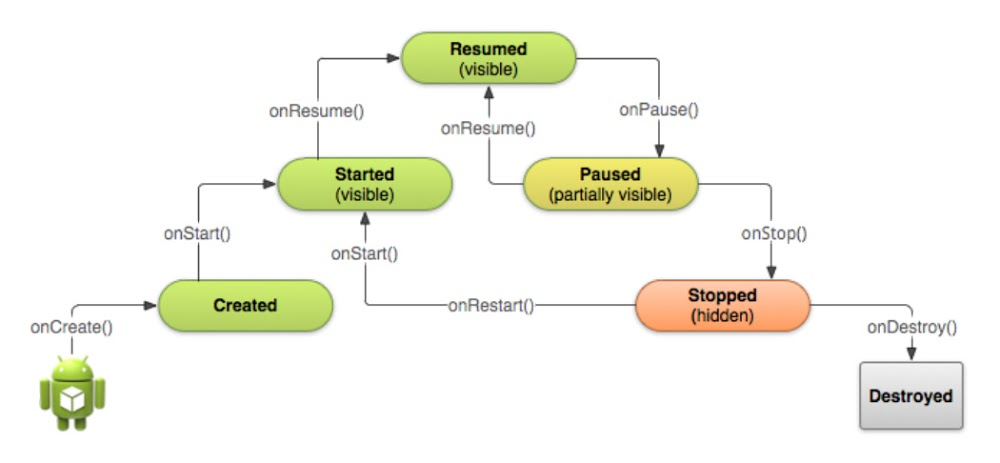
\includegraphics[width=0.8\columnwidth]{Figures/2/lifecycle}
		\caption{วัฏจักรของแอคทิวิตี้บนระบบปฏิบัติการแอนดรอยด์}{ที่มา : https://www.dev2qa.com/android-activity-lifecycle-example/}
		\label{Fig:lifecycle}
	\end{figure}
	จากรูปที่ \ref{Fig:lifecycle} แสดงวัฏจักรของแอคทิวิตี้ในรูปแบบโครงสร้างพีระมิดโดยแสดงให้เห็นว่า Method ที่เรียกใช้
	งานอัตโมัติ (Callback Method) ได้แก่ onCreate(), onStart(), onResume() และ onRestart() จะขยับแอคทิวิตี้ขึ้นไปด้านบนสุดที่ Resumed Method
	และมี Method ได้แก่ onPause(), onStop() และ onDestroy() ที่จะขยับแอคทิวิตี้ลงมาด้านล่าง แอคทิวิตี้ยังสามารถกลับไปทำงานที่ตำแหน่ง Resumed Method จากตำแหน่ง Paused และ Stopped ได้อีกด้วย
	
	ในบางครั้งไม่จำเป็นต้องเรียกใช้งาน Callback Method ทั้งหมดเสมอไปขึ้นกับความซับซ้อนของแอคทิวิตี้ อย่างไรก็ตามเป็นสิ่งสำคัญที่นักพัฒนาควรทำความเข้าใจแต่ละ Method เพื่อให้มั่นใจได้ว่าแอปพลิเคชันของที่ได้พัฒนาตอบสนองเป็นไปตามที่ผู้ใช้คาดหวัง ดังนั้น ในการใช้งาน Callback Method
	ที่ถูกวิธีก็จะช่วยให้แอปพลิเคชันทำงานได้เป็นอย่างดี ดังนี้
	\begin{itemize}
		\item ไม่หยุดการทำงานหรือค้าง กรณีมีสายโทรเข้าหรือมีการสลับไปใช้งานแอปพลิเคชันอื่น 
		\item ไม่ใช้ทรัพยากรที่มีค่าของระบบอย่างสูญเปล่า ถ้าไม่มีการใช้งานแอคทิวิตี้ใดๆ 
		\item ไม่กระทบต่อกระบวนการในขั้นตอนการใช้งานของผู้ใช้กรณีออกจากแอปพลิเคชันแล้วกลับเข้ามาใช้งานอีกครั้ง 
		\item ไม่หยุดการทำงานหรือระบบค้างที่กระทบการใช้งานของผู้ใช้กรณีมีการหมุนหน้าจอแนวนอนและแนวตั้งสลับกัน
	\end{itemize}
	
	เหตุการณ์ที่แอคทิวิตี้มีการเปลี่ยน Method ต่าง ๆ ตามแสดงในรูปที่  \ref{Fig:lifecycle}
	แต่มีอยู่ 3 Method เท่านั้นที่แอคทิวิตี้จะยังคงอยู่คงที่ในช่วงเวลาระยะเวลาหนึ่งไม่เปลี่ยนไป Method อื่นในทันที ได้แก่
		\begin{itemize}
		\item Resumed (แสดงอยู่ ทำงานอยู่) ใน Method นี้แอคทิวิตี้จะแสดงอยู่ด้านหน้าสุดและผู้ใช้กำลังใช้งานอยู่ บ่อยครั้งจะเรียกว่า Running Method
		\item Paused (แสดงหน้าจอบางส่วน ไม่ถูกบังสนิท) ใน Method นี้แอคทิวิตี้จะถูกบดบังด้วยแอคทิวิตี้อื่น เช่น แอคทิวิตี้อื่นที่อยู่ด้านหน้าสุดที่แสดงในลักษณะกึ่งโปรงใสหรือไม่ได้แสดงแบบเต็มหน้าจอ  แอคทิวิตี้ในสถานะนี้จะไม่สามารถรับค่าจากผู้ใช้และทำงานคำสั่งใด ๆ ได้
		\item Stopped (แสดงหน้าจอแบบ Background ผู้ใช้มองไม่เห็น) ใน Method นี้ แอคทิวิตี้จะถูกบดบังอย่างสมบูรณ์และผู้ใช้มองไม่เห็นโดยจะถูกย้ายไปอยู่ด้านหลังในขณะที่อยู่ใน Method นี้
		ค่า Activity Instance และตัวแปรทั้งหมดจะยังคงอยู่แต่จะไม่สามารถถูกเรียกมาใช้งานจากโค้ดใด ๆ ได้
		\end{itemize}
		ในขณะที่ Method อื่น เช่น Created และ Started จะแสดงชั่วคราวแล้วระบบก็จะเปลี่ยนไป Method อื่นในทันทีที่ Method ถูกเรียกใช้งานอัตโนมัติ นั่นคือ หลังจากที่ระบบเรียกใช้งาน onCreate() แล้วก็จะเรียกใช้งาน onStart()
		ทันทีและสุดท้ายตามด้วย onResumne()  ซึ่งก็จะเข้าสู่ Resumed Method ทั้งหมดก็คือวัฏจักรแอคทิวิตี้เบื้องต้น

	 \section{ความรู้พื้นฐาน Ionic Framework}
	 Ionic Framework คือเครื่องมือในการสร้าง Mobile Application เป็นเครื่องมือสร้างแอปมือถือที่สามารถสร้างทีเดียว สามารถใช้งานได้บนระบบปฏิบัติการ 
	 iOS, Android และ Windows ซึ่งก็จะใช้งานร่วมกับ Framework ตัวอื่น ๆ ได้ คือ Angular และ Apache Cordova 
	 ในตอนสุดท้าย เพื่อให้ทั้งแอปที่เขียนมาใช้ได้กับทุกระบบปฏิบัติการ

		\subsection{เทคโนโลยีที่ใช้ในการพัฒนา Ionic Framework}
		Ionic Framework พัฒนา Frontend ด้วยภาษา HTML , CSS , JavaScript และถูก Build เป็น Application ด้วย Cordova
		\item HTML5  คือ คือ ภาษามาร์กอัป ที่ใช้สำหรับเขียน website ซึ่ง HTML5 นี้เป็นภาษาที่ถูกพัฒนาต่อมาจากภาษา HTML และพัฒนาขึ้นมาโดย WHATWG (The Web Hypertext Application Technology Working Group) โดยได้มีการปรับเพิ่ม Feature หลายๆอย่างเข้ามาเพื่อให้ผู้พัฒนาสามารถใช้งานได้ง่ายมากยิ่งขึ้น
		\item CSS3  คือ สไตล์ชีท เป็นภาษาที่ใช้เป็นส่วนของการจัดรูปแบบการแสดงผลของ HTML พูดง่ายๆ คือทำให้การแสดงผลของ HTML ให้สวยงาม
		\item AngularJs คือ JavaScript Framework  รูปแบบหนึ่งที่พัฒนามาจาก Google หน้าที่ของมันคือเป็น engine ที่ใช้ควบคุมในส่วน front end ของเว็บได้เป็นอย่างดีมีการทำงานแบบ Model View Controller (MVC)
		
		\begin{figure}[H]
			\centering
			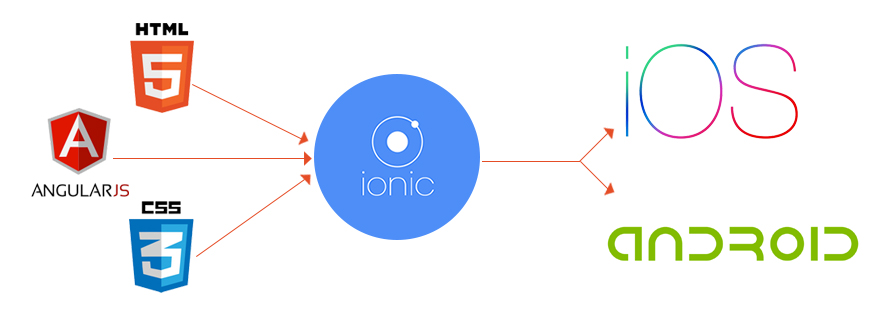
\includegraphics[width=0.8\columnwidth]{Figures/2/ionic1}
			\caption{การทำงานของ Ionic Framework}{ที่มา : http://blog.prscreative.com/what-is-ionic/}
			\label{Fig:lifecycle}
		\end{figure}

		\subsection{การทำงานของ Cordova Application}
		\begin{figure}[H]
			\centering
			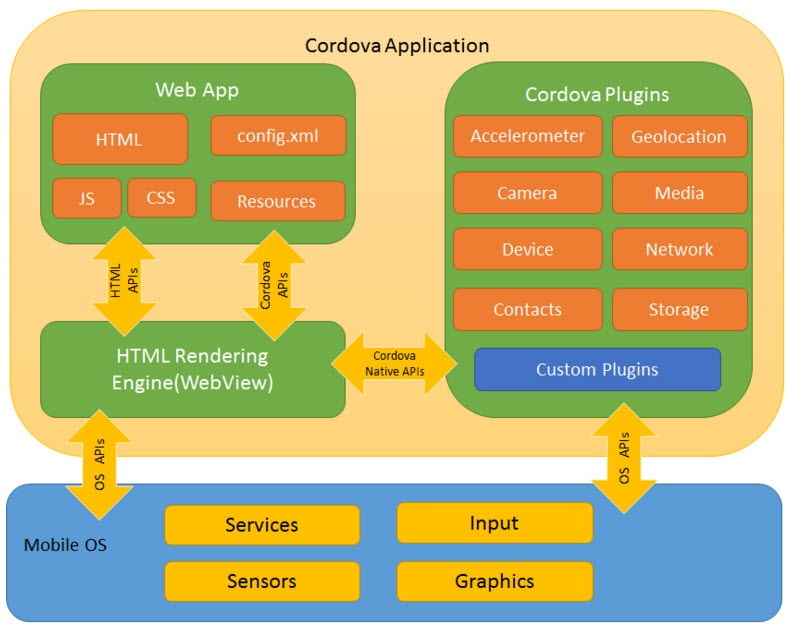
\includegraphics[width=0.8\columnwidth]{Figures/2/ionic2}
			\caption{Cordova Application}{ที่มา : http://blog.prscreative.com/what-is-ionic/}
			\label{Fig:lifecycle}
		\end{figure}
		\begin{figure}[H]
			\centering
			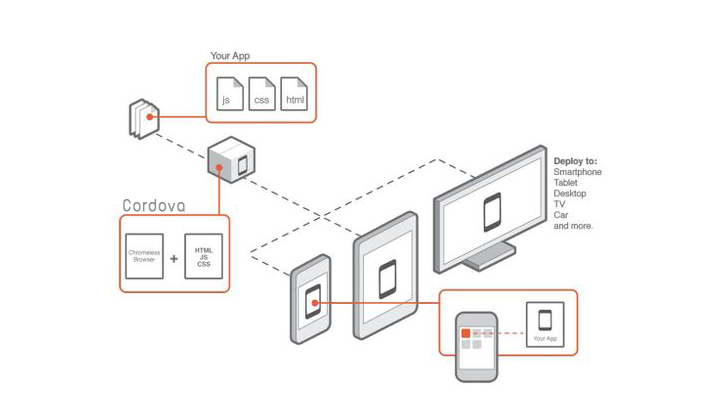
\includegraphics[width=0.8\columnwidth]{Figures/2/ionic3}
			\caption{Cordova Build Application}{ที่มา : http://blog.prscreative.com/what-is-ionic/}
			\label{Fig:lifecycle}
		\end{figure}

		\item Cordova มีหน้าที่ห่อหุ้มแอปพลิเคชันไว้ และทำหน้าที่ติดต่อกับ Hardware ของ Mobile เป็นหลักเพราะมี API ติดต่อกับ Hardware โดยตรง เช่น Camera, Contacts, Media, Network
		
		\subsection{ความแตกต่างระหว่าง PhoneGap/Cordova}
		PhoneGap และ Cordova มีลักษณะคล้ายกัน เนื่องจากมันเกือบจะเหมือนกัน ต่างกันเพียงเรื่องของลิขสิทธิ์ และการนำไปใช้งาน
		\item PhoneGap : ในยุคแรกถูกพัฒนาโดย Nitobi เปิดให้ใช้งานแบบ Open Source ซึ่งได้รับความนิยมในการนำมาใช้เป็นเทคโนโลยี Hybrid ซึ่งต่อมาถูกซื้อโดยบริษัท Adobe เพื่อนำมาเสริมทัพให้กับโปรแกรม Adobe Dreamweaver เพื่อให้สั่ง Build app จากโปรแกรม Dreamweaver ให้ลองรับหลาย Platform ได้ แต่มีค่าลิขสิทธิ์โปรแกรม
		\item Cordova : เกิดขึ้นจากการตกลงกันระหว่าง Adobe และ Nitobi ด้วยแนวคิดที่อยากให้ PhoneGap เป็น Open Source ต่อไป จึงได้มีการตกลงกันให้นำโค๊ดของ PhoneGap ไปตั้งเป็นชื่อใหม่ นั่นก็คือ Cordova เพื่อมอบให้ Apache Foundation ไปดูแลถูกนำไปใช้ในโครงการ Hybrid mobile application หลายโครงการ เช่น AppGyver, Ionic framework
		 




	\section{การใช้งาน Firebase เป็นฐานข้อมูล}
	Firebase \cite{bib9} คือ บริการ Backend และ แพลตฟอร์ม ครบวงจรสำหรับนักพัฒนาแอปพลิเคชัน และโปรแกรมประยุกต์บนเว็บแพลตฟอร์มที่มีเครื่องมือและโครงสร้างพื้นฐานที่ได้รับการออกแบบมาเพื่อช่วยให้นักพัฒนาสามารถสร้างแอปพลิเคชันพลิเคที่มีคุณภาพสูง Firebase (ไฟร์เบส) ถูกสร้างขึ้นจากคุณสมบัติเสริมว่านักพัฒนาสามารถผสมและจับคู่เพื่อให้พอดีกับความต้องการของตน บริษัท ก่อตั้งขึ้นในปี 2011 โดยแอนดรูลีและเจมส์ เทมปลิน สินค้าเริ่มต้น Firebase) เป็นฐานข้อมูลเรียลไทม์ซึ่งมี API ที่ช่วยให้นักพัฒนาในการจัดเก็บและซิงค์ข้อมูล ดังรูป \ref{Fig:class1}
	
	Google Firebase 2.0 มีการพัฒนาจากบริการ Backend เก็บข้อมูลอย่างเดียว มาเป็น แพลตฟอร์มครบวงจรสำหรับนักพัฒนาแอปพลิเคชัน (รองรับ iOS, Android, Web) และรองรับบริการทุกอย่างที่นักพัฒนาแอปต้องการใช้งาน
	
	\begin{figure}[H]
		\centering
		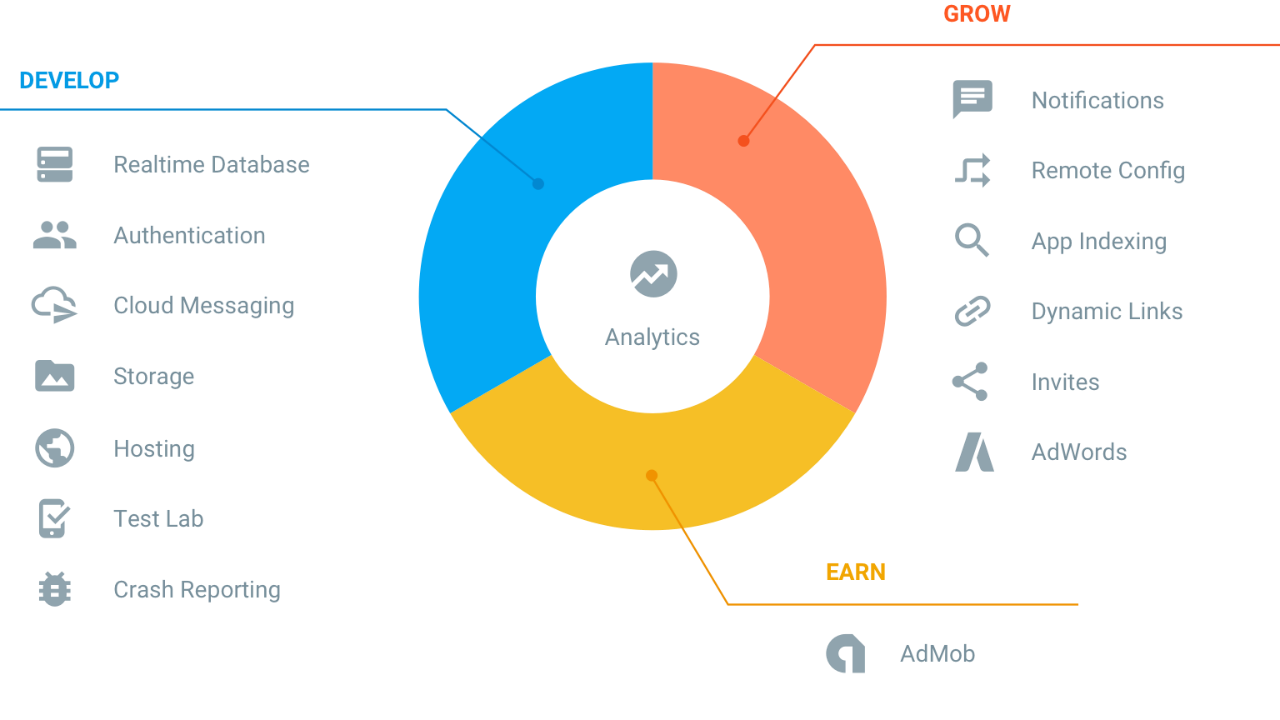
\includegraphics[width=\columnwidth]{Figures/2/firebase}
		\caption{Firebase 2.0}{ที่มา : www.mindphp/คู่มือ/73-คืออะไร/3921-what-is-firebase-backend.html}
		\label{Fig:class1}
	\end{figure}
\subsection{บริการหลักของไฟร์เบส}
\begin{itemize}
	\item Realtime Database จัดเก็บและซิงค์ข้อมูลระหว่างผู้ใช้และอุปกรณ์ต่างๆแบบเรียลไทม์โดยใช้ฐานข้อมูล NoSQL ที่โฮสต์บนระบบคลาวด์ ซิงค์ข้อมูลที่อัปเดตระหว่างอุปกรณ์ที่เชื่อมต่อเป็นมิลลิวินาทีและข้อมูลจะยังคงมีอยู่ถ้าแอพพลิเคชันออฟไลน์
	\item Authentication จัดการบัญชีผู้ใช้ด้วย Firebase Auth ซึ่งใช้งานง่ายและปลอดภัยมีวิธีการหลายในการสร้างบัญชีผู้ใช้และตรวจสอบความถูกต้อง ได้แก่ อีเมล/รหัสผ่าน, ผู้ให้บริการบุคคลที่สามเช่น Google หรือ Facebook 
	\item Cloud Storage จัดเก็บภาพเสียงวิดีโอหรือเนื้อหาอื่น ๆ เช่น รูปภาพโปรไฟล์ผู้ใช้ หรือวีดีทัศน์ต่างๆ เป็นต้น ซึ่งมีความปลอดภัยในการอัปโหลดไฟล์และดาวน์โหลดสำหรับแอพพลิเคชัน
	\item Hosting ใช้ในการเผยแพร่เว็บไซต์  โดยเนื้อหาภายในเว็บเป็นเดชบอร์ด รายงานข้อต่างๆ ของผู้ใช้ ซึ่งต้องทำการเข้าสู่ระบบก่อน
	\item Crashlytics เป็นบริการล่าสุดที่กูเกิลได้เข้าควบรวมเข้ามาไว้ในบริการไฟร์เบส สามารถรายงานข้อขัดข้องได้อย่างมีประสิทธิภาพ เปิดใช้งานการวิเคราะห์แบบเรียลไทม์เพื่อช่วยให้เข้าใจสิ่งที่เกิดขึ้นในแอพพลิเคชัน เครื่องมือวิเคราะห์ข้อมูลจะให้ข้อมูลเชิงลึก
	\item Cloud Firestore เป็นบริการในส่วนของ Database ที่ใช้ระบบฐานของข้อมูลแบบ NoSQL ที่เป็นแบบ Document Database และเป็นการนำเอาข้อดีต่างๆของบริการด้านฐานข้อมูลของ Realtime Database มาปรับปรุงพัฒนาต่อและเพิ่มความสามารถขึ้นไปมากขึ้น ซึ่งผู้เขียนจะได้กล่าวถึงในบทถัดไป
\end{itemize}
\subsection{การพัฒนา Cloud Firestore}
การพัฒนา Cloud Firestore แบ่งออกแบบ 5 ขั้นตอน ดังนี้
\begin{enumerate}
	\item การสร้าง Cloud Firestore เพื่อใช้งานในโครงการ ในขั้นตอนแรกทำการสร้าง Database เพื่อที่จะใช้งาน Cloud Firestore ก่อน โดยใช้บัญชี Gmail ต่อมาเข้าไปที่เว็บ https://firebase.google.com  ดังรูปภาพที่ \ref{Fig:f1}
	\begin{figure}[H]
		\centering
		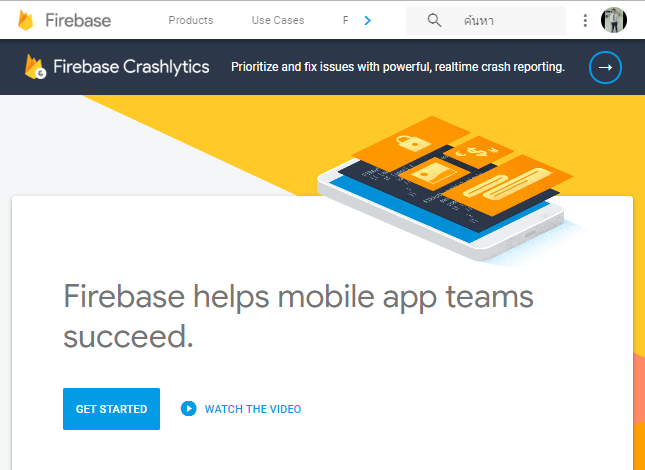
\includegraphics[width=0.7\columnwidth]{Figures/2/f1}
		\caption{เว็บ https://firebase.google.com}{ที่มา :https://medium.com/20scoops-cnx/เข้มข้นกับ-firebase-cloud-firestore-ระบบฐานข้อมูลที่เปิดตัวใหม่ล่าสุดจาก-firsbase-แบบจัดเต็ม-d001e43e2be7 }
		\label{Fig:f1}
	\end{figure}
	\item ติดตั้ง SDKs เพื่อใช้งาน Cloud Firestore
	โดย SDKs ที่ Firebase ได้เตรียมไว้ให้ สามารถดูรายละเอียดได้ที่ https://firebase.google.com/docs/firestore/quickstart
	\item ออกแบบโครงสร้างและการจัดการข้อมูล  
	\begin{itemize}
		\item  ระบบฐานข้อมูลของ Cloud Firestore จะเป็น NoSQL แบบ Document ซึ่งจะแตกต่างจากระบบฐานข้อมูลแบบ SQL โดยจะไม่มีตาราง ไม่มีแถว แต่เก็บข้อมูล ภายใน Document จะเก็บแบบ Key-value โดยแต่ละ Document จะถูกเก็บไว้ใน Collection ซึ่งใน Document สามารถมี Subcollection ได้
		\item Collection เป็นการเรียกชื่อแทนของการเก็บหลายๆเอกสารไว้ด้วยกัน เช่น เก็บข้อมูลของ User จำนวนมากไว้ด้วยกัน จึงตั้งชื่อ Collection ว่า Users ซึ่งใน Collection เดียวกันผู้ใช้งานสามารถใส่ข้อมูลที่แตกต่างชนิดกันในแต่ละ Key แต่ละ Document ได้ โดยในแต่ละ Key และ Document จะมีอิสระในการใส่ข้อมูล แต่ควรใส่ข้อมูลในแต่ละ Key ของ Document เป็นประเภทเดียวกันเพราะจะทำให้การค้นหาและการจัดเรียงลำดับของข้อมูลนั้นง่ายขึ้น
		\item Subcollection สามารถสร้าง Subcollection ของ Subcollection ไปได้เรื่อยๆ โดย Cloud Firestore ว่าสามารถซ้อนกันไปได้ 100 ลำดับชั้น
	\end{itemize}
	\item การรับและสอบถามข้อมูล
	การรับและสอบถามข้อมูลจาก Cloud Firestore จะมี 2 วิธี โดยจะสามารถใช้ได้ทั้งการรับข้อมูลและการสอบถามข้อมูล
	\begin{itemize}
		\item การรับข้อมูลเพียงครั้งเดียวจะเป็นการรับข้อมูลเมื่อมีจุดประสงค์ที่จะไม่ต้องการรับรู้การเปลี่ยนแปลงของข้อมูล ซึ่ง ณ ขณะนั้นข้อมูลมีค่าเป็นอะไรก็จะได้ค่านั้นมา หากมีการเปลี่ยนแปลงข้อมูลในภายหลัง ผู้ใช้งานต้องเป็นผู้จัดการรับข้อมูลล่าสุดเอง โดยวิธีการรับข้อมูลเพียงครั้งเดียวจะใช้ Method Get()
		\item การรับข้อมูลแบบ Realtime update จะเป็นการรับข้อมูลเมื่อผู้ใช้งานมีจุดประสงค์ที่จะต้องการรับรู้การเปลี่ยนแปลงของข้อมูล ซึ่ง ณ ขณะที่ข้อมูลเกิดการเปลี่ยนแปลงจะมีการรับข้อมูลที่เกิดการเปลี่ยนแปลงโดยอัตโนมัติ โดยในครั้งแรกที่มีการรับข้อมูลจะสร้าง Initialize Instance และทุกครั้งที่ข้อมูลมีการเปลี่ยนแปลงก็จะส่ง Callback ให้กับ Iistener โดยผ่าน Method onSnapshot()
	\end{itemize}
	\item การป้องกันและความปลอดภัยของข้อมูลข้อมูลใน Cloud Firestore ได้มีการออกแบบให้สามารถกำหนดกฏของความปลอดภัยต่างๆได้ โดยผ่าน Firebase Console  ซึ่งหากใช้ Cloud Firestore ผู้ใช้งานสามารถมาทำเรื่องการป้องกันและรักษาความปลอดภัยของข้อมูลเพียงที่เดียวก็สามารถใช้ได้ทั้งหมดไม่ว่าจะเป็น Web และ Mobile ส่วนฝั่ง Server ก็สามารถใช้ IAM ใน Google Cloud Platform มาจัดการความปลอดภัยสำหรับ Cloud Firestore ได้
\end{enumerate}


\section{ความรู้พื้นฐานของแชทบอท}
Chatbot คือโปรแกรมคอมพิวเตอร์ชนิดหนึ่ง ถูกพัฒนาขึ้นมาให้มีบทบาทในการตอบกลับการสนทนาด้วยตัวอักษรแบบอัตโนมัติผ่าน Messaging Application เสมือนการโต้ตอบของคนจริง ๆ หรืออาจเรียกง่าย ๆ ว่า โปรแกรมตอบกลับอัตโนมัติ ซึ่งเวลานี้กลายเป็นสุดยอดผู้ช่วยอัจฉริยะที่ทุกบริษัทต้องการนำมาใช้กับธุรกิจออนไลน์ ในการสื่อสารกับกลุ่มลูกค้าแบบเรียลไทม์

วิธีเลือกข้อความในการตอบกลับของแชทบอท จะขึ้นอยู่กับชนิดของแชทบอทด้วย ทั้งการใช้ระบบ Database บันทึกคำถามและคำตอบเอาไว้จำนวนหนึ่ง แล้วตรวจจับ Keyword จากคำถามเพื่อประมวลคำตอบส่งกลับไปหาลูกค้า (Rule-based Chatbot) แต่ถ้าเป็นแชทบอทที่มีความซับซ้อน โต้ตอบเลียนแบบการสนทนาของคนจริง ๆ ได้ จะใช้ปัญญาประดิษฐ์ (AI) ในการประมวลผล ซึ่งต้องใช้เงินลงทุนในการพัฒนาค่อนข้างสูง

การพัฒนาระบบหุ่นยนต์โต้ตอบสนทนาอัตโนมัติ (Chatbot Agent) นั้น, สามารถทำได้โดยการแปลงคำพูดของผู้ใช้ที่ใช้ภาษาธรรมชาติ อาทิเช่น ภาษาไทยหรือภาษาอังกฤษ (Query) ให้เป็นข้อมูลที่สามารถประมวลผลได้ (Intent). โดยที่การแปลงนี้ (Intent Classification) เกิดขึ้นเมื่อผู้ใช้ป้อนข้อมูล ที่ใกล้เคียงหรือตรงกับกับข้อมูลคำพูด (Training Phase) ของหนึ่งในเจตนา (Intent) ที่นักพัฒนาโปรแกรมกำหนดไว้. เจตนาเหล่านั้นเป็นหัวข้อที่ใช้ดำเนินการตามคำพูดของผู้ใช้

หุ่นยนต์โต้ตอบอัตโนมัติสามารถออกแบบมาเพื่อจัดการการสนทนา ด้วยความช่วยเหลือจากข้อมูลบริบท (Context), ลำดับความสำคัญของเจตนา (Intent Priority), การดึงข้อมูลสำคัญจากคำพูดของผู้ใช้ (Action and Parameters). นอกจากนี้ยังเปิดให้นักพัฒนาเขียนโปรแกรม (Code) เสริมเพื่อการประมวลผลเพิ่มเติมได้ ผ่านช่องทางเชื่อมต่อต่างๆ อาทิเช่น Webhook หรือ Fulfillment. ซึ่งแผนภาพต่อไปนี้แสดงการจัดการคำขอของผู้ใช้เมื่อมีผู้ใช้ส่งคำพูดมายังระบบหุ่นยนต์โต้ตอบสนทนาอัตโนมัติ

\begin{figure}[H]
	\centering
	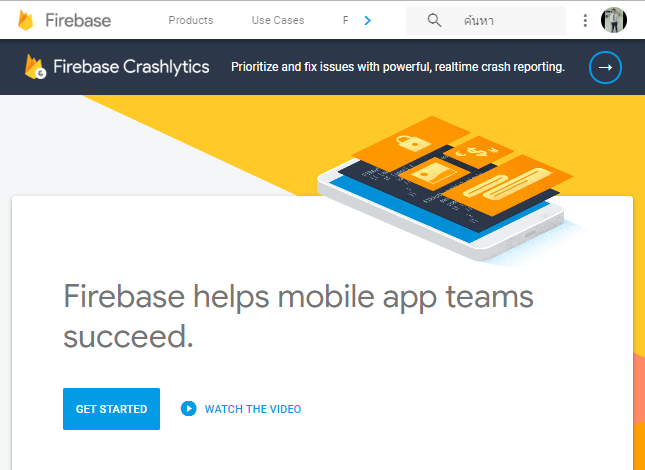
\includegraphics[width=0.7\columnwidth]{Figures/2/f1}
	\caption{รูปแบบการส่งข้อมูลผู้ใช้ไปยังแชทบอท}{ที่มา :https://kobkrit.com/การพัฒนาระบบหุ่นยนต์โต้ตอบสนทนาอัตโนมัติภาษาไทย-chatbot-ด้วย-dialogflow-1-529c308b25ec}
	\label{Fig:f1}
\end{figure}

เมื่อผู้ใช้ส่งข้อความมาผ่านโปรแกรมสนทนา (Chat Messenger) หรือเสียงผ่านไมโครโฟน (Microphone) จากอุปกรณ์ต่างๆ ซึ่งเสียงจะถูกแปลงเป็นข้อความด้วยโปรแกรมรู้จำคำพูด (Speech Recognition) แล้วนั้น. ข้อความคำพูดของผู้ใช้เหล่านี้ (Query) ก็จะถูกแปลงเป็นหัวข้อเจตนา (Intent) โดยใช้เทคนิคทางปัญญาประดิษฐ์ที่ใช้คัดแยกเจตนาจากคำพูด (Intent Classification). โดยใช้ทำงานของโปรแกรมคัดแยกเจตนาจากคำพูดนั้น จะใช้หลักการเทียบความเหมือนกับความคล้ายของคำพูดของผู้ใช้ ว่าใกล้เคียงกับกลุ่มคำพูดตัวอย่างของเจตนานั้น (Training Phase) ซึ่งกำหนดไว้ล่วงหน้านั้นๆหรือไม่} โดยการพิจารณาหัวข้อเจตนา (Intent) ที่เหมาะสมนั้น เราสามารถใช้บริบท (Context) เป็นตัวกำหนดว่าเจตนาไหนจะถูกนำมาพิจารณาในการคัดเลือกบ้าง. โดยที่หากเจตนาไหนไม่ตรงกับบริบทที่กำหนดไว้ ก็จะไม่ถูกคัดเลือก ไม่ว่าจะมีกลุ่มคำพูดตัวอย่างใกล้เคียงกับคำพูดของผู้ใช้มากแค่ไหนก็ตาม

หลังจากที่คัดเลือกเจตนาได้แล้ว, ระบบก็จะสามารถเลือกคำตอบที่เหมาะสม ซึ่งกำหนดไว้โดยนักพัฒนาระบบหุ่นยนต์โต้ตอบสนทนาอัตโนมัติ. ซึ่งอาจจะเป็นคำตอบตายตัว (Static Response) หรือ คำตอบแบบพลวัต (Dynamic Response) ที่สร้างจากการประมวลโปรแกรมเพิ่มเติม เขียนโดยนักพัฒนาเชื่อมต่อกับระบบหุ่นยนต์โต้ตอบสนทนาอัตโนมัติ (Chatbot Agent) ผ่านช่องทาง API (Fulfillment) ก็ได้. โดยนักพัฒนาระบบหุ่นยนต์โต้ตอบสนทนาอัตโนมัตินั้น สามารถเชื่อมหุ่นยนต์กับบริการ API ภายนอกอื่นๆ (External APIs). ซึ่งเป็นการเปิดช่องทางให้หุ่นยนต์ก็สามารถเชื่อมต่อกับระบบฐานข้อมูลภายนอกใดๆ (RDMS) ก็ได้. สามารถนำช่องทางนี้มาใช้การดึงหรือบันทึกข้อมูล ให้สามารถสร้างคำตอบข้อมูลแบบพลวัต ตรงตามความต้องการของผู้ใช้ได้อีกด้วย

หลังจากนั้น ข้อความตอบกลับของผู้ใช้ก็จะถูกส่งกลับไปยังโปรแกรมสนทนา หรือตอบกลับเป็นเสียงผ่านลำโพงผ่านโปรแกรมสังเคราะห์เสียง (Speech Synthesis) ไปยังอุปกรณ์ต่างๆได้อีกด้วย ทำให้ครบองค์ประกอบการสนทนาระหว่างมนุษย์และหุ่นยนต์ ซึ่งขั้นตอนโดยสรุปนั้นก็คือ

\begin{enumerate}
	\item รับเข้าคำสนทนาจากมนุษย์ผ่านข้อความโดยตรง หรือข้อความรู้จำจากเสียงมนุษย์โดยใช้เทคโนโลยีรู้จำเสียงพูด (Speech Recognition)
	\item คัดแยกเจตนาจากคำพูด (Intent Classification) โดยพิจารณาจากกลุ่มคำพูดตัวอย่าง (Training Phase) และบริบท (Context)
	\item เมื่อเราได้เจตนาแล้วเราก็สามารถสร้างคำตอบที่เหมาะสมด้วยการไปดึงคำตอบที่กำหนดไว้ (Static Response) ของเจตนานั้นๆ. หรือ ส่งออกเป็นคำตอบแบบพลวัต (Dynamic Reponse) ซึ่งสร้างด้วยการประมวลผลโค้ด (Code) โดยสามารถไปดึงข้อมูลภายนอกที่ต้องการจะใช้จากฐานข้อมูลหรือบริการภายนอกต่างๆด้วยช่องทาง Fulfillment
	\item ส่งคำตอบไปยังมนุษย์ โดยอาจจะเป็นข้อความหรือเป็นเสียงก็ได้ ผ่านเทคโนโลยีการสังเคราะห์เสียงจากข้อความ (Speech Synthesis)
\end{enumerate}

\section{Dialogflow}
Dialogflow คือ platform สำหรับสร้าง chatbot ของ Google ที่ใช้ machine learning ด้าน Natural Language Processing (NLP) มาช่วยในทำความเข้าใจถึงความต้องการ (intent) และสิ่งที่ต้องการ (entity) ในประโยคสนทนาของผู้ใช้งาน และตอบคำถามตามความต้องการของผู้ใช้งาน ตามกฎ หรือ flow ที่ผู้พัฒนาวางเอาไว้ ซึ่ง Dialogflow จะช่วยเพิ่มความยืดหยุ่นของประโยคที่ chatbot รับมา ว่าไม่จำเป็นต้องตรงตามเงื่อนไข แบบ rule based ก็สามารถเข้าใจถึงความต้องการของผู้ใช้งานได้


\section{Libraries moment.js}
moment.js คือ javascript library สำหรับใช้สำหรับจัดการ Date และ Time ที่จะช่วยอำนวยความสะดวกในเรื่องการจัด Format Date ให้ตรงกับที่เราต้องการ
มี Feature ที่หลากหลายครอบคลุมทั้งใช้งาน Format ทั้ง Date , Time , Timezone , Standard Time , Local Time เป็นต้น ซึ่งการนำ library moment.JavaScript 
มาใช้งานสามารถติดตั้งได้ดังนี้
\begin{enumerate}
	\item คำสั่งในการติดตั้ง
	\begin{figure}[H]
		{\setstretch{1.0}\begin{lstlisting}
			/*  install dependency */
			npm install moment --save   # npm
			yarn add moment             # Yarn
			Install-Package Moment.js   # NuGet
			spm install moment --save   # spm
			meteor add momentjs:moment  # meteor
			bower install moment --save # bower (deprecated)
		\end{lstlisting}}
	\centering
		\caption{คำสั่งในการติดตั้ง moment.js}
		\label{Fig:API Web Speech}
	\end{figure}
	\item วิธีการเรียกใช้งาน moment.js \\ รู้จักการเรียกใช้งาน moment แบบง่าย ๆ เรียก moment() จะได้ datetime ปัจจุบัน อยากจะเปลี่ยน format ก็เรียก function format(‘format string’) ก็จะได้ format ตามต้องการ
	\begin{figure}[H]
		{\setstretch{1.0}\begin{lstlisting}
			const moment = require('moment');

			const SLASH_DMY = 'DD/MM/YYYY';
			const SLASH_DMYHMS = 'DD/MM/YYYY HH:mm:ss';
			const SLASH_YMD = 'YYYY/MM/DD';
			const SLASH_YMDHMS = 'YYYY/MM/DD HH:mm:ss';
			const DASH_DMY = 'DD-MM-YYYY';
			const DASH_DMYHMS = 'DD-MM-YYYY HH:mm:ss';
			const DASH_YMD = 'YYYY-MM-DD';
			const DASH_YMDHMS = 'YYYY-MM-DD HH:mm:ss';
			
			console.log('sysdate ::==',moment());
			
			console.log('sysdate ::==',moment().format(SLASH_DMY));
			console.log('sysdate ::==',moment().format(SLASH_DMYHMS));
			
			console.log('sysdate ::==',moment().format(SLASH_YMD));
			console.log('sysdate ::==',moment().format(SLASH_YMDHMS));
			
			console.log('sysdate ::==',moment().format(DASH_DMY));
			console.log('sysdate ::==',moment().format(DASH_DMYHMS));
			
			console.log('sysdate ::==',moment().format(DASH_YMD));
			console.log('sysdate ::==',moment().format(DASH_YMDHMS));
			/*
			sysdate ::== moment("2018-07-03T21:08:38.248")
			sysdate ::== 03/07/2018
			sysdate ::== 03/07/2018 21:08:38
			sysdate ::== 2018/07/03
			sysdate ::== 2018/07/03 21:08:38
			sysdate ::== 03-07-2018
			sysdate ::== 03-07-2018 21:08:38
			sysdate ::== 2018-07-03
			sysdate ::== 2018-07-03 21:08:38
			*/
		\end{lstlisting}}
	\centering
		\caption{การเรียกใช้งาน moment.js}
		\label{Fig:API Web Speech}
	\end{figure}
	การเปลี่ยน format ของ String date ทำได้โดยส่งเป็น parameter เข้า function moment(‘my_date’) ก็จะได้ moment object เราก็จะสามารถทำไปใช้งานต่อได้ แต่มีข้อสังเกตุ การใช้งาน DateTime เรื่อง TimeZone ของแต่ละภูมิภาคที่ต่างกันทำให้ moment แจ้ง warning วิธีแก้เบื้องต้นก็ให้กำหนด input format ของ ข้อมูลส่งเข้าเพื่อบอกให้ moment รู้
	\begin{figure}[H]
		{\setstretch{1.0}\begin{lstlisting}
			const moment = require('moment');

const my_date = '2017/07/03';

console.log('not pass input format ::==',moment(my_date).format('DD/MM/YYYY'));
/*
Deprecation warning: value provided is not in a recognized RFC2822 or ISO format. moment construction falls back to js Date(), which is not reliable across all browsers and versions. Non RFC2822/ISO date formats are discouraged and will be removed in an upcoming major release. Please refer to http://momentjs.com/guides/#/warnings/js-date/ for more info.
Arguments:
[0] _isAMomentObject: true, _isUTC: false, _useUTC: false, _l: undefined, _i: 2017/07/03, _f: undefined, _strict: undefined, _locale: [object Object]
Error
    at Function.createFromInputFallback (D:\Skill\momentJS\node_modules\moment\moment.js:320:98)
    at configFromString (D:\Skill\momentJS\node_modules\moment\moment.js:2368:15)
    at configFromInput (D:\Skill\momentJS\node_modules\moment\moment.js:2594:13)
    at prepareConfig (D:\Skill\momentJS\node_modules\moment\moment.js:2577:13)
    at createFromConfig (D:\Skill\momentJS\node_modules\moment\moment.js:2544:44)
    at createLocalOrUTC (D:\Skill\momentJS\node_modules\moment\moment.js:2631:16)
    at createLocal (D:\Skill\momentJS\node_modules\moment\moment.js:2635:16)
    at hooks (D:\Skill\momentJS\node_modules\moment\moment.js:12:29)
    at Object.<anonymous> (D:\Skill\momentJS\myMoment.js:30:42)
    at Module._compile (module.js:652:30)
not pass input format ::== 03/07/2017
*/

console.log('pass input format ::==',moment(my_date,'YYYY/MM/DD').format('DD/MM/YYYY'));
/*
pass input format ::== 03/07/2017
*/
		\end{lstlisting}}
	\centering
		\caption{การเรียกใช้งาน moment.js}
		\label{Fig:API Web Speech}
	\end{figure}

\end{enumerate}


















	\section{ความรู้พื้นฐานของระบบ XX เดิม}
		 \subsection{ความเป็นมา}

      ระบบ XX เดิม มีประวัติดังนี้ 
		  
		  \subsection{วิสัยทัศน์และพันธกิจ}
		  \begin{itemize}
			  \item วิสัยทัศน์ (Vision)
			  "เป็นองค์กรหลักที่ XX"
			  
			  \item พันธกิจ (Mission)
			  \begin{enumerate}
			  	\item สนับสนุนและส่งเสริม XX 
			  	\item พัฒนาองค์กรสู่ความเป็นเลิศด้วยนวัตกรรมที่ทันสมัย โดยใช้หลักบริหารจัดการที่ดี
			  \end{enumerate}
		  \end{itemize}
	  
	  \subsection{ขั้นตอนการดำเนินการ XX}
	  \begin{itemize}
	  	\item อธิบายขั้นตอนที่ XX
	  	\item อธิบายขั้นตอนที่ XX
	  	\item อธิบายขั้นตอนที่ XX
	  \end{itemize}
	  

	\section{เอกสารและงานวิจัยที่เกี่ยวข้อง}
		  กล่าวถึงเอกสาร งานวิจัย หรือระบบงานที่คล้ายกันโดยแบ่งเป็น subsection โดยแต่ละหัวข้อให้อธิบายความสำคัญ ฟังก์ชันการทำงาน ข้อจำกัดหรือข้อแตกต่างจะระบบที่จะทำ เช่น
		 \subsection{เว็บไซต์ XX}
		 PSU Studentloan \cite{PSU} เป็นเว็บไซต์ที่ให้บริการนักศึกษากองทุนเงินให้กู้ยืมเพื่อการศึกษา มหาวิทยาลัยสงขลานครินทร์ วิทยาเขตหาดใหญ่ สามารถเข้าใช้งานได้ที่ https://studentloan.psu.ac.th/home มีฟังก์ชันการทำงานพื้นฐานอันได้แก่ การดูข่าวสารประชาสัมพันธ์  ประมวลภาพกิจกรรม ดาวน์โหลดเอกสารที่เกี่ยวข้อง เป็นต้น
			 \begin{figure}[H]
			 	\centering
			 	
\includegraphics[width=0.8\textwidth]{Figures/2/1}
			 	\caption{หน้าแรกของเว็บไซต์ PSU Studentloan}{ที่มา : https://studentloan.psu.ac.th/home}
			 	\label{Fig:Studentloan1}
			 \end{figure}
			 
		 \subsection{แอปพลิเคชัน XX}
		 eStudentloan \cite{eStudentloan} เป็นแอนดรอย์แอปพลิเคชันที่พัฒนาโดยฝ่ายกิจการนักศึกษา สถาบันเทคโนโลยีไทย-ญี่ปุ่น เพื่อให้บริการนักศึกษากองทุนเงินให้กู้ยืมเพื่อการศึกษาสถาบันเทคโนโลยีไทย-ญี่ปุ่น สามารถดาวน์โหลดเพื่อใช้งานได้ที่  https://play.google.com/store/apps/details?id=th.co.dest.anek.studentloan โดยแอปพลิเคชันมีฟังก์ชันการทำงาน คือ ติดตามข่าวสารจากหน่วยงาน 
		 \newpage
	 			\begin{figure}[H]
	 				\centering
	 				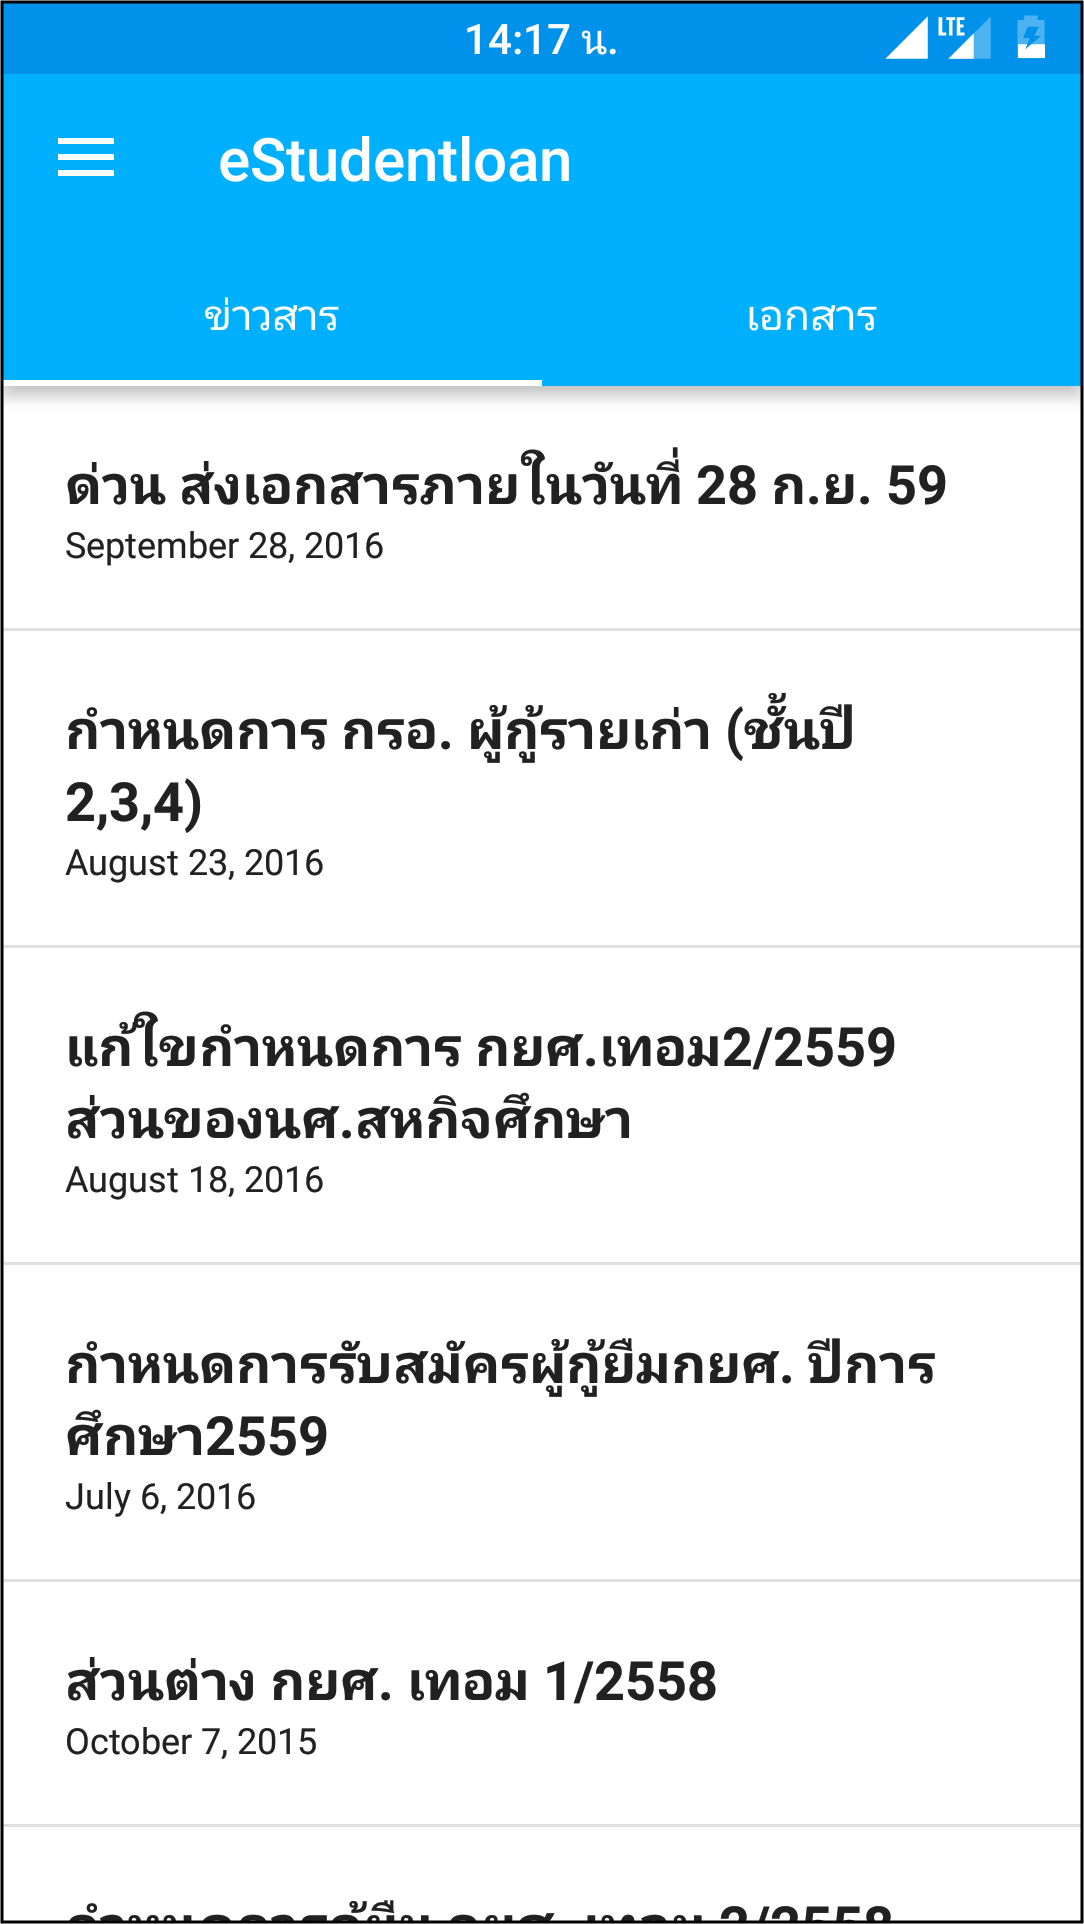
\includegraphics[width=0.45\textwidth]{Figures/2/m3}
	 				\caption{ข่าวสารจากหน่วยงาน}{ที่มา : https://play.google.com/store/apps/details?id=th.co.dest.anek.studentloan}
	 				\label{Fig:Studentloan11}
	 			\end{figure}
	
